\chapter{Espacios métricos}
\begin{definition}[Espacio métrico]
Un \textbf{espacio métrico} es un par $\displaystyle \left(X, d\right) $ donde $\displaystyle X $ es un conjunto no vacío y $\displaystyle d : X \times X \to \R $ es una función que se llama \textbf{distancia} o \textbf{métrica}, tal que:
\begin{enumerate}
\item $\displaystyle d\left(x,y\right) \geq 0 $, $\displaystyle \forall x,y \in X $.
\item $\displaystyle d\left(x,y\right) = 0 \iff x = y $.
\item $\displaystyle d\left(x,y\right) = d\left(y,x\right) $, $\displaystyle \forall x,y \in X $.
\item (Propiedad triangular) $\displaystyle d\left(x,y\right) \leq d\left(x,z\right) + d\left(z,y\right) $, $\displaystyle \forall x,y,z \in X $.
\end{enumerate}
\end{definition}
\begin{eg} Algunos ejemplos de espacios métricos son:
\begin{enumerate}
\item Consideremos $\displaystyle \left(\R, d\right) $ donde $\displaystyle d\left(x,y\right) = \left|x - y\right| $.
\item La distancia euclídea en $\displaystyle \R^{2} = \left\{ \left(x,y\right) \; : \; x,y \in \R\right\} $: 
	\[ d\left(\left(x_{1}, x_{2}\right), \left(y_{1}, y_{2}\right)\right) = \sqrt{\left(x_{1}-y_{1}\right)^{2}+\left(x_{2}-y_{2}\right)^{2}}.\]
\item La 'métrica del taxi' en $\displaystyle \R^{2} $ con distancia:
	\[d _{1}\left(\left(x_{1}, x_{2}\right), \left(y_{1}, y_{2}\right)\right) = \left|x_{1} - y_{1}\right| + \left|x_{2}-y_{2}\right| .\]
\item Distancias geodésicas: el camino más corto (por ejemplo, en una superficie esférica el camino más corto entre dos puntos es un arco de circunferencia).
\item Distancias en $\displaystyle \R^{n} $. Si $\displaystyle x = \left(x_{1}, \ldots, x_{n}\right) $ e $\displaystyle y= \left(y_{1}, \ldots, y_{n}\right) $, consideramos la distancia euclídea
	\[d _{2}\left(x,y\right) = \sqrt{\left(x_{1}-y_{1}\right)^{2} + \cdots + \left(x_{n}-y_{n}\right)^{2}} .\]
También podemos generalizar la 'métrica del taxi':
\[ d _{1}\left(x,y\right) = \left|x_{1}-y_{1}\right| + \cdots + \left|x_{n}-y_{n}\right| .\]
También se puede considerar la métrica
\[d _{\infty}\left(x,y\right) = \max \left\{  \left|x_{i}-y_{i}\right| \; : \; 1 \leq i \leq n\right\}  .\]
\end{enumerate}
\end{eg}
\begin{definition}[Espacio discreto]
Sea $\displaystyle X \neq \emptyset $ un conjunto cualquiera, y definimos $\displaystyle \forall x,y \in X $ 
\[d\left(x,y\right) = 
\begin{cases}
0, \; \text{si} \; x = y \\
1, \; \text{si} \; x \neq y
\end{cases}
.\]
Se dice que $\displaystyle d $ es la \textbf{métrica discrecta} y $\displaystyle \left(X, d\right) $ el \textbf{espacio métrico discreto}.
\end{definition}
\begin{definition}[Subespacio métrico]
Sea $\displaystyle \left(X, d\right) $ un espacio métrico y sea $\displaystyle Y \subset X $. Se define la \textbf{métrica relativa} (o \textbf{restringida}) a $\displaystyle Y $ como $\displaystyle d _{Y}\left(y, y'\right)  = d\left(y, y'\right) $, $\displaystyle \forall y, y' \in Y $. Entonces, $\displaystyle \left(Y, d _{Y}\right) $ es un espacio métrico que llamaremos \textbf{subespacio} de $\displaystyle X $.
\end{definition}
\section{Espacios normados}
\begin{definition}[Espacio normado]
Un \textbf{espacio normado} es un par $\displaystyle \left(E, \left\| \cdot \right\|\right) $ donde $\displaystyle E $ es un espacio vectorial y $\displaystyle \| \cdot \| : E \to \R $ es una función que se llama \textbf{norma} tal que:
\begin{enumerate}
\item $\displaystyle \| x \| \geq 0 $, $\displaystyle \forall x \in E $.
\item $\displaystyle \| x \| = 0 \iff x = 0 $.
\item $\displaystyle \| \lambda x \| = \left|\lambda \right|\|x\| $, $\displaystyle \forall \lambda \in \K, \forall x \in E $ \footnote{En este curso $\displaystyle \K $ va a ser principalmente $\displaystyle \R $.}.
\item $\displaystyle \| x + y \| \leq \| x \| + \| y \|$, $\displaystyle \forall x,y \in E $.
\end{enumerate}
\end{definition}
\begin{prop}
Sea $\displaystyle \left(E, \| \cdot \|\right) $ un espacio normado. Si definimos 
\[d\left(x,y\right) = \| x- y\|, \forall x,y \in E ,\]
se obtene que $\displaystyle d $ es una distancia en $\displaystyle E $, que se llama \textbf{asociada} a la norma. 
\end{prop}
\begin{proof}
Demostremos todas las propiedades de las métricas:
\begin{enumerate}
\item Tenemos que $\displaystyle d\left(x,y\right) = \|x-y\| \geq 0 $, $\displaystyle \forall x,y \in E $.
\item $\displaystyle d\left(x,y\right) = 0 \iff \|x-y\|=0\iff x - y = 0 \iff x = y $.
\item $\displaystyle d\left(x,y\right) = \|y - x\| = \left|-1\right| \|x-y\| = \|x-y\| = d\left(x,y\right) $.
\item $\displaystyle d\left(x,y\right) = \| x- y\| = \|x-z + z- y\| \leq \|x - z\| + \|z - y\| = d\left(x,z\right) + d\left(z,y\right) $.
\end{enumerate}
\end{proof}
\begin{observation}
En $\displaystyle \R^{n} $, dado $\displaystyle x = \left(x_{1}, \ldots, x_{n}\right) \in \R^{n} $ se definen:
\[ \text{(Norma euclídea)} \quad \|x\|_{2} = \sqrt{x^{2}_{1} + \cdots + x^{2}_{n}} .\]
\[\|x\|_{1} = \left|x_{1}\right| + \cdots + \left|x_{n}\right| .\]
\[ \|x\|_{\infty} = \max \left\{ \left|x_{i}\right| \; : \; 1 \leq i \leq n\right\}  .\]
\end{observation}
\begin{prop}[Relación entre las normas en $\displaystyle \R^n $]
$\displaystyle \forall x = \left(x_{1}, \ldots, x_{n}\right) \in \R^{n} $, 
\[ \|x\| _{\infty} \leq \|x\|_{2} \leq \|x\|_{1} \leq n\|x\|_{\infty} .\]
\end{prop}
\begin{proof}
Supongamos que $\displaystyle \left|x_{i_{0}}\right| = \|x\|_{\infty} $. Entonces, tenemos que
\[ \displaystyle \left|x_{i_{0}}\right|^{2} \leq \left|x_{1}\right|^{2} + \cdots + \left|x_{n}\right|^{2}.\]
Dado que la función de la raíz es creciente, tenemos que 
\[ \|x\|_{\infty} = \left|x_{i_{0}}\right| \leq \sqrt{\left|x_{1}\right|^{2} + \cdots + \left|x_{n}\right|^{2}} = \|x\|_{2}.\]
Por otro lado, tenemos que
\[ \|x\|_{1}^{2} = \left(\left|x_{1}\right| + \cdots + \left|x_{n}\right|\right)^{2}= \left|x_{1}\right|^{2} + \cdots + \left|x_{n}\right|^{2} + C \footnote{ $\displaystyle C \geq 0. $}  \geq \left|x_{1}\right|^{2} + \cdots + \left|x_{n}\right|^{2} = \|x\|_{2}^{2} .\]
Finalmente, tenemos que 
\[ \|x\|_{1} = \left|x_{1}\right| + \cdots + \left|x_{n}\right| \leq \left|x_{i_{0}}\right| + \cdots + \left|x_{i_{0}}\right| = n \left|x_{i_{0}}\right| = n \|x\|_{\infty} .\]
\end{proof}
\begin{definition}
Dos normas $\displaystyle \| \cdot \| $ y $\displaystyle \| \cdot \|' $ en un mismo espacio vectorial $\displaystyle E $ son \textbf{equivalentes} cuando existen $\displaystyle m, M > 0 $ tales que 
\[m \|x\|' \leq \|x\| \leq M \|x\|', \; \forall x \in E .\]
\end{definition}
\begin{observation}
Hemos visto en la proposición anterior que $\displaystyle \| \cdot\|_{1}, \| \cdot \|_{2} $ y $\displaystyle \| \cdot \|_{\infty} $ son equivalentes en $\displaystyle \R^{n} $.
\end{observation}
\begin{definition}[Producto escalar]
Sea $\displaystyle E $ un espacio vectorial real. Un \textbf{producto escalar} en $\displaystyle E $ es una forma bilineal, simétrica y definida positiva. Es decir, una aplicación $\displaystyle \left\langle ,  \right\rangle : E \times E \to \R $ tal que 
\begin{enumerate}
\item $\displaystyle \left\langle \lambda x + \mu y, z \right\rangle = \lambda \left\langle x, z \right\rangle +\mu \left\langle y, z \right\rangle  $, $\displaystyle \forall x,y,z \in E, \forall \lambda, \mu \in \R $. 
\item $\displaystyle \left\langle x, y \right\rangle = \left\langle y, x \right\rangle  $, $\displaystyle \forall x,y \in E $.
\item $\displaystyle \forall x\in E $, $\displaystyle \left\langle x, x \right\rangle \geq 0 $ y $\displaystyle \left\langle x, x \right\rangle = 0 \iff x = 0 $.
\end{enumerate}
\end{definition}
\begin{observation}
En este caso, denotaremos $\displaystyle \|x\| = \sqrt{\left\langle x, x \right\rangle } $.
\end{observation}

\begin{theorem}[Desigualdad de Cauchy-Schwarz]
Sea $\displaystyle E $ un espacio vectorial dotado de un producto escalar $\displaystyle \left\langle ,  \right\rangle  $. Entonces
\[|\left\langle x, y \right\rangle| \leq \| x \| \cdot \|y\|, \; \forall x,y \in E .\]
\end{theorem}
\begin{proof}
\begin{description}
\item[Caso 1.] Si $\displaystyle x = 0 $ o $\displaystyle y = 0 $, obtenemos la igualdad.
\item[Caso 2.] Si $\displaystyle y \neq 0 $, tenemos que $\displaystyle \forall \alpha \in \R $,
	\[0 \leq \left\langle x + \alpha y, x + \alpha y \right\rangle = \left\langle x, x \right\rangle +\alpha \left\langle x, y \right\rangle +\alpha \left\langle y, x \right\rangle +\alpha ^{2}\left\langle y, y \right\rangle  = \|x\|^{2} + 2\alpha \left\langle x, y \right\rangle +\alpha ^{2} \|y\|^{2} .\]
	Tomamos $\displaystyle \alpha = -\frac{\left\langle x, y \right\rangle }{\|y\|^{2}} $. Así, tenemos que 
	\[
	\begin{split}
		0 & \leq \|x\|^{2} - \frac{2\left\langle x, y \right\rangle ^{2}}{\|y\|^{2}} + \frac{\left\langle x, y \right\rangle ^{2}}{\|y\|^{4}}\|y\|^{2} = \|x\|^{2} - \frac{\left\langle x, y \right\rangle ^{2}}{\|y\|^{2}} .
	\end{split}
	\]
Así, tenemos que $\displaystyle \frac{\left\langle x, y \right\rangle ^{2}}{\|y\|^{2}} \leq \|x\|^{2} $, por lo que $\displaystyle \left\langle x, y \right\rangle ^{2} \leq \|x\|^{2}\|y\|^{2} $ y tenemos que $\displaystyle \left|\left\langle x, y \right\rangle \right| \leq \|x\|\|y\| $.	
\end{description}
\end{proof}
\begin{prop}
Sea $\displaystyle E $ un espacio vectorial dotado de un producto escalar $\displaystyle \left\langle ,  \right\rangle  $. Entonces, $\displaystyle \|x\| = \sqrt{\left\langle x, x \right\rangle } $, es una norma en $\displaystyle E $, que se dice asociada a $\displaystyle \left\langle ,  \right\rangle  $.
\end{prop}
\begin{proof}
Comprobamos que se cumplen las propiedades de las normas:
\begin{enumerate}
\item Tenemos que claramente $\displaystyle \|x\| = \sqrt{\left\langle x, x \right\rangle } \geq 0 $, $\displaystyle \forall x \in E $.
\item $\displaystyle \|x\| = 0 \iff \left\langle x, x \right\rangle = 0 \iff x = 0$.
\item $\displaystyle \|\lambda x\|^{2} = \left\langle \lambda x, \lambda x \right\rangle = \lambda ^{2} \left\langle x, x \right\rangle = \lambda ^{2} \|x\|^{2} $. Tomando la raíz cuadrada, $\displaystyle \|\lambda x\| = \left|\lambda \right|\|x\| $.
\item Si $\displaystyle x,y \in E $,
	\[
	\begin{split}
		\|x + y \|^{2} = & \left\langle x + y, x+y \right\rangle = \|x\|^{2} + 2\left\langle x, y \right\rangle + \|y\|^{2}\\
		\leq & \|x\|^{2} + 2\|x\|\|y\| + \|y\|^{2} = \left(\|x\| + \|y\|\right)^{2}.
	\end{split}
	\]
	Tomando raíces, tenemos que se verifica la propiedad triangular: $\displaystyle \|x + y\| \leq \|x\| + \|y\| $.
\end{enumerate}
\end{proof}
\section{Bolas en un espacio métrico}
\begin{definition}
Sea $\displaystyle \left(X, d\right) $ un espacio métrico y consideramos $\displaystyle a \in X $, $\displaystyle r > 0 $. Se definen como \textbf{bola abierta} de centro $\displaystyle a $ y radio $\displaystyle r $ al conjunto 
\[B\left(a,r\right) = \left\{ x \in X \; : \; d\left(x,a \right) < r\right\}  .\]
Similarmente, se llama \textbf{bola cerrada} de centro $\displaystyle a $ y radio $\displaystyle r $ al conjunto 
\[\overline{B}\left(a,r\right) = \left\{ x \in X \; : \; d\left(x,a\right) \leq r\right\}  .\]
\end{definition}
\begin{eg}
Considermos bolas en $\displaystyle \R^{2} $ de distintas normas. 
\begin{enumerate}
\item Consideremos bolas abiertas y cerradas con la métrica euclídea: 
	\[ B_{2}\left(\left(0,0\right), r\right) = \left\{ \left(x,y\right) \; : \; \sqrt{x ^{2} + y^{2}} < r\right\}, \; \overline{B}_{2}\left(\left(0,0\right), r\right) = \left\{ \left(x,y\right) \; : \; \sqrt{x^{2} +y^{2}} \leq r\right\}.\]
\begin{center}
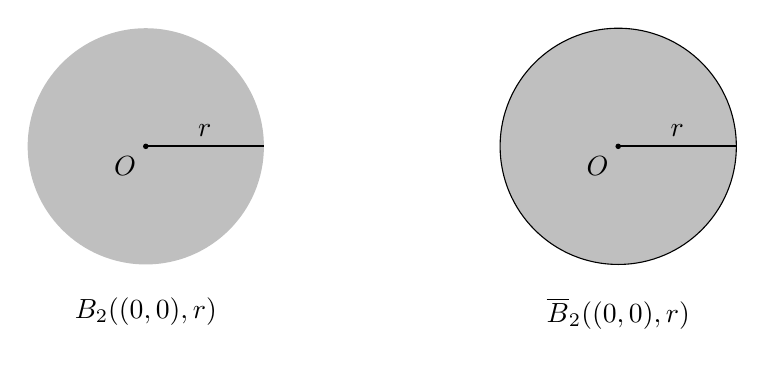
\begin{tikzpicture}

%--- Open ball: B_2((0,0),r) ---
\begin{scope}[shift={(-3,0)}] % shift left
  % Open ball (filled only, no border)
  \fill[gray!50] (0,0) circle (1.5); % radius = r

  % Origin
  \fill (0,0) circle (1pt);
  \node[below left] at (0,0) {$O$};

  % Radius line
  \draw[thick] (0,0) -- (1.5,0) node[midway, above] {$r$};

  % Label below
  \node[below] at (0,-1.8) {$B_2((0,0),r)$};
\end{scope}

%--- Closed ball: \overline{B}_2((0,0),r) ---
\begin{scope}[shift={(3,0)}] % shift right
  % Closed ball (filled + border)
  \filldraw[fill=gray!50, draw=black] (0,0) circle (1.5); % radius = r

  % Origin
  \fill (0,0) circle (1pt);
  \node[below left] at (0,0) {$O$};

  % Radius line
  \draw[thick] (0,0) -- (1.5,0) node[midway, above] {$r$};

  % Label below
  \node[below] at (0,-1.8) {$\overline{B}_2((0,0),r)$};
\end{scope}

\end{tikzpicture}
\end{center}

\item Consideremos bolas abiertas y cerradas con la métrica 'del taxi': 
	\[ B_{1}\left(\left(0,0\right), r\right) = \left\{ \left(x,y\right) \; : \; \left|x\right| + \left|y\right| < r\right\} , \; \overline{B}_{1}\left(\left(0,0\right), r\right) = \left\{ \left(x,y\right) \; : \; \left|x\right| + \left|y\right| \leq r\right\}.\]
	\begin{center}
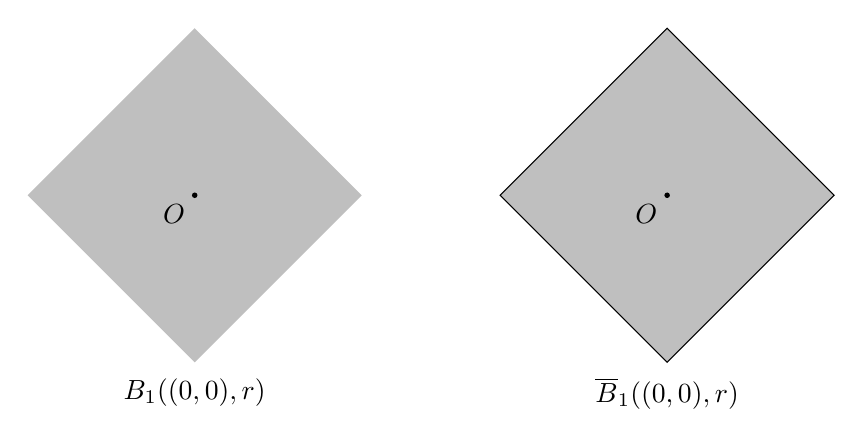
\begin{tikzpicture}
%--- Open L1 ball: B_1((0,0),r) ---
\begin{scope}[shift={(-3,0)}, rotate=45] % left, rotated 45 degrees
  % Filled square, no border
  \fill[gray!50] (-1.5,-1.5) rectangle (1.5,1.5);
  % Origin
  \fill (0,0) circle (1pt);
  \node[below left] at (0,0) {$O$};
\end{scope}
\node[below] at (-3,-2.2) {$B_1((0,0),r)$};
%--- Closed L1 ball: \overline{B}_1((0,0),r) ---
\begin{scope}[shift={(3,0)}, rotate=45] % right, rotated 45 degrees
  % Filled square, with border
  \filldraw[fill=gray!50, draw=black] (-1.5,-1.5) rectangle (1.5,1.5);
  % Origin
  \fill (0,0) circle (1pt);
  \node[below left] at (0,0) {$O$};
\end{scope}
\node[below] at (3,-2.2) {$\overline{B}_1((0,0),r)$};
\end{tikzpicture}	
	\end{center}
	
\item Consideremos bolas abiertas y cerradas con la métrica infinita:
	\[ B_{\infty}\left(\left(0,0\right), r\right) = \left\{ \left(x,y\right) \; : \; \max \left\{ \left|x\right|, \left|y\right|\right\} < r\right\} = \left\{ \left(x,y\right) \; : \; \left|x\right|, \left|y\right| < r\right\} .\]
	\[\overline{B}_{\infty}\left(\left(0,0\right), r\right) = \left\{ \left(x,y\right) \; : \; \max \left\{ \left|x\right|, \left|y\right|\right\} \leq r\right\} = \left\{ \left(x,y\right) \; : \; \left|x\right|, \left|y\right| \leq r\right\}  .\]
\begin{center}
	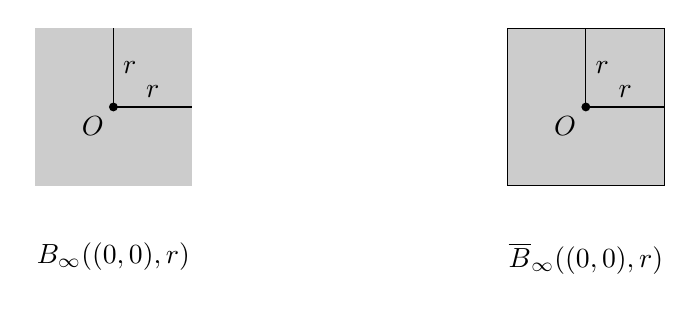
\begin{tikzpicture}[scale=2]

%--- Open L∞ ball: B∞((0,0),r) ---
\begin{scope}[shift={(-1.5,0)}] % shift left, closer
  % Square (filled only, no border)
  \fill[gray!40] (-0.5,-0.5) rectangle (0.5,0.5);

  % Origin
  \fill (0,0) circle (0.8pt);
  \node[below left] at (0,0) {$O$};

  % Radius lines
  \draw (0,0) -- (0,0.5) node[midway,right] {$r$};
  \draw (0,0) -- (0.5,0) node[midway,above] {$r$};

  % Label
  \node[below] at (0,-0.8) {$B_{\infty}((0,0),r)$};
\end{scope}

%--- Closed L∞ ball: \overline{B}∞((0,0),r) ---
\begin{scope}[shift={(1.5,0)}] % shift right, closer
  % Square (filled + border)
  \filldraw[fill=gray!40, draw=black] (-0.5,-0.5) rectangle (0.5,0.5);

  % Origin
  \fill (0,0) circle (0.8pt);
  \node[below left] at (0,0) {$O$};

  % Radius lines
  \draw (0,0) -- (0,0.5) node[midway,right] {$r$};
  \draw (0,0) -- (0.5,0) node[midway,above] {$r$};

  % Label
  \node[below] at (0,-0.8) {$\overline{B}_{\infty}((0,0),r)$};
\end{scope}

\end{tikzpicture}
\end{center}
	
\end{enumerate}
\end{eg}
\begin{observation}
	En $\displaystyle \left(\R, \left| \cdot \right|\right) $ se tiene que $\displaystyle B\left(0,r\right) = \left(-r,r\right) $ y $\displaystyle \overline{B}\left(0,r\right) = \left[-r,r\right]  $. Similarmente, tenemos que $\displaystyle B\left(a,r\right) = \left(a-r, a + r\right) $ y $\displaystyle \overline{B}\left(a,r\right) = \left[a - r, a + r\right]  $.
\end{observation}
\begin{observation}[Relación de las bolas en $\displaystyle \R^n $]
Sabemos que 
\[\|x\|_{\infty} \leq \|x\|_{2} \leq \|x\|_{1} \leq n \|x\|_{\infty} .\]
Por tanto, tenemos que 
\[B_{1}\left(a,r\right) \subset B_{2}\left(a,r\right) \subset B_{\infty}\left(a,r\right) \subset B_{1}\left(a, nr\right) \footnote{También se puede escribir $\displaystyle B_{\infty}\left(a,nr\right) \subset B_{1}\left(a,r\right) \subset B_{2}\left(a,r\right) \subset B_{\infty}\left(a,nr\right) $ .}  .\]
En efecto, si $\displaystyle x \in B_{1} \left(a,r\right) $, tenemos que $\displaystyle \|x - a\|_{1} < r $. Por tanto, es fácil ver que $\displaystyle \|x - a\|_{2} \leq \|x - a\|_{1} < r $, por lo que $\displaystyle x \in B_{2}\left(a,r\right) $. El resto de inclusiones se deducen de forma análoga.
\end{observation}
\begin{definition}
Sean $\displaystyle \left(X,d\right) $ un espacio métrico y $\displaystyle A \subset X $. Se define el \textbf{diámetro} de $\displaystyle A $ como 
\[diam\left(A\right) = \sup \left\{ d\left(x,y\right) \; : \; x,y \in A\right\} \in [0, \infty) .\]
Se dice que $\displaystyle A $ es \textbf{acotado} si $\displaystyle diam\left(A\right) < \infty $.
\end{definition}
\begin{prop}
Dado un espacio métrico $\displaystyle \left(X,d\right) $ con $\displaystyle A \subset X $, tenemos que $\displaystyle A $ está acotado si y solo si $\displaystyle A $ está contenido en alguna bola.
\end{prop}
\begin{proof}
\begin{description}
\item[(i)] Supongamos que $\displaystyle A $ está acotado, entonces $\displaystyle diam\left(A\right) = r < \infty $. Así, tenemos que si $\displaystyle x \in A $, etonces $\displaystyle \forall a \in A $ se tiene que $\displaystyle d\left(a,x\right) \leq r $, por lo que $\displaystyle A \subset \overline{B}\left(a,r\right) $. También podemos ver que lo contiene una bola abierta: $\displaystyle A \subset \overline{B}\left(a, r\right) \subset B\left(a, r+1\right) $.
\item[(ii)] Si $\displaystyle A $ está contenido en una bola, tenemos que existe $\displaystyle x \in X $ y $\displaystyle \frac{r}{2}>0 $ tal que $\displaystyle A \subset B\left(x, \frac{r}{2}\right) $. De esta manera, si $\displaystyle a,b \in A $ se tiene que 
	\[d\left(a,b\right) \leq d\left(a,x\right) + d\left(x,b\right) < \frac{r}{2} + \frac{r}{2} = r .\]
	Así, se tiene que $\displaystyle \forall a,b \in A $, $\displaystyle d\left(a,b\right) < r $, por lo que $\displaystyle diam\left(A\right) \leq r < \infty $, por lo que $\displaystyle A $ está acotado.
\end{description}
\end{proof}

\section{Conceptos topológicos}
\begin{definition}[Conjunto abierto]
Sean $\displaystyle \left(X,d\right) $ un espacio métrico y $\displaystyle A \subset X $. Se dice que $\displaystyle A $ es un \textbf{conjunto abierto} si $\displaystyle \forall a \in A, \exists r> 0 $ tal que $\displaystyle B\left(a,r\right) \subset A $.
\end{definition}
\begin{prop}
Toda bola abierta es un conjunto abierto.
\end{prop}
\begin{proof}
	Tomemos $\displaystyle A = B\left(a,R\right) $ y $\displaystyle x \in B\left(a,R\right) $. Sea $\displaystyle \delta = d\left(x, a\right) < R $ y $\displaystyle r = R - \delta > 0 $ \footnote{No hace falta de escribir $\displaystyle r = \min \left\{ R - \delta, \delta \right\} $ al tratarse de una bola.}. Sea $\displaystyle y \in B\left(x,r\right) $, tenemos que $\displaystyle d\left(x,y\right) < r $. Así, 
\[d\left(y,a\right) \leq d\left(y,x\right) + d\left(x,a\right) < r + \delta = R .\]
Así, $\displaystyle y \in B\left(a,R\right) $, por lo que $\displaystyle B\left(x,r\right) \subset B\left(a,R\right) $.
\end{proof}
\begin{eg}
En $\displaystyle \left(\R^{2}, \| \cdot \|_{2}\right) $.
\begin{enumerate}
	\item Consideremos $\displaystyle A = \left\{ \left(x,y\right) \; : \; 0 < x < 1\right\}  $. Vamos a ver que es abierto. Si $\displaystyle a \in A $, sea $\displaystyle a = \left(x,y\right) $ y consideramos $\displaystyle r = \min \left\{ x, 1 - x\right\}  $. Entonces, tenemos que $\displaystyle B_{2}\left(a,r\right) \subset A $, en efecto, si $\displaystyle \left(x', y'\right) \in B_{2}\left(a,r\right) $:
\[\sqrt{\left(x-x'\right)^{2} + \left(y-y'\right)^{2}} < r \Rightarrow \left|x - x'\right| < r \Rightarrow 0 < x' < 1.\]
Así, tenemos que $\displaystyle \left(x',y'\right)\in A $.
\item Consideremos $\displaystyle A = \left\{ \left(x,y\right) \; : \; 0 < x \leq 1\right\}  $. Vamos a ver que no es abierto. En efecto, si tomamos $\displaystyle a = \left(1,0\right) $ y $\displaystyle r > 0 $,
	tenemos que $\displaystyle \left(1 + \frac{r}{2}, 0\right) \in B_{2}\left(a,r\right) $ pero $\displaystyle \left(1 + \frac{r}{2}, 0\right) \not\in A $. 
\end{enumerate}
\end{eg}
\begin{prop}
En $\displaystyle \R^{n} $ los conjuntos abiertos coinciden para $\displaystyle \| \cdot \|_{1} $, $\displaystyle \| \cdot \|_{2} $ y $\displaystyle \| \cdot \|_{\infty} $.
\end{prop}
\begin{proof}
Como se vio en una observación anterior, sabemos que 
\[B_{1}\left(a,r\right) \subset B_{2}\left(a,r\right) \subset B_{\infty}\left(a,r\right) \subset B_{1}\left(a,nr\right) .\]
\begin{itemize}
\item Sea $\displaystyle A \subset \R^{n} $. Si $\displaystyle A $ es abierto con la norma $\displaystyle \| \cdot \|_{2} $, tenemos que $\displaystyle \forall a \in A, \exists r > 0 $ tal que $\displaystyle B_{2}\left(a,r\right) \subset A $. Por la observación, como $\displaystyle B_{1}\left(a,r\right) \subset B_{2}\left(a,r\right) \subset A $, tenemos que también es abierto para la norma $\displaystyle \| \cdot \|_{1} $.
\item Sea $\displaystyle A \subset \R^{n} $. Si $\displaystyle A $ es abierto con la norma $\displaystyle \| \cdot \|_{\infty} $, entonces $\displaystyle \forall a \in A, \exists r > 0 $ tal que $\displaystyle B_{\infty}\left(a,r\right) \subset A $. Por la observación anterior, tenemos que $\displaystyle B_{2}\left(a,r\right) \subset B_{\infty}\left(a,r\right) \subset A $, por lo que $\displaystyle A $ es abierto respecto a la norma $\displaystyle \| \cdot \|_{2} $.
\item Sea $\displaystyle A \subset \R^{n} $. Si $\displaystyle A $ es abierto respecto de $\displaystyle \| \cdot \|_{1} $, tenemos que $\displaystyle \forall a \in A, \exists r > 0 $ tal que $\displaystyle B_{1}\left(a,r\right) \subset A $. Sea $\displaystyle r' = \frac{r}{n} > 0 $, 
	\[B_{\infty}\left(a,r'\right)\subset B_{1}\left(a, nr'\right) = B_{1}\left(a,r\right) \subset A.\]
	Por tanto, $\displaystyle A $ es abierto respecto de la norma $\displaystyle \| \cdot \| _{\infty} $.
\end{itemize}
\end{proof}
\begin{theorem}[Propiedades de los abiertos]
Sea $\displaystyle \left(X,d\right) $ un espacio métrico. 
\begin{enumerate}
\item $\displaystyle X $ y $\displaystyle \emptyset $ son abiertos.
\item La unión arbitraria de abiertos es abierto.
\item La intersección finita de abiertos es abierto.
\end{enumerate}
\end{theorem}
\begin{proof}
\begin{enumerate}
\item Es trivial que $\displaystyle \emptyset $ es abierto. Por otro lado, si $\displaystyle a \in X $, tenemos que $\displaystyle \forall r > 0 $, $\displaystyle B\left(x,r\right) \subset X $. Así, $\displaystyle X $ está abierto.
\item Supongamos que $\displaystyle \left\{ A_{i}\right\}_{i \in I} $ es una familia de conjuntos abiertos y sea $\displaystyle A = \bigcup_{i \in I}A_{i} $. Si $\displaystyle a \in A $, tenemos que $\displaystyle a \in A_{i} $ para algún $\displaystyle i \in I $. Así, existe $\displaystyle r>0 $ tal que $\displaystyle B \left(a,r\right) \subset A_{i} \subset \bigcup_{i \in I}A_{i}$. Por tanto, $\displaystyle B\left(a,r\right) \subset A $ y $\displaystyle A $ es abierto.
\item Sean $\displaystyle A_{1}, \ldots, A_{m} $ conjuntos abiertos y sea $\displaystyle A = A_{1} \cap \cdots \cap A_{m} $. Si $\displaystyle a \in A $, tenemos que $\displaystyle a \in A_{i} $ para $\displaystyle 1 \leq i \leq m $.
	Así, existe $\displaystyle r_{i} > 0 $ tal que $\displaystyle B\left(a, r_{i}\right) \subset A_{i} $. Si tomamos $\displaystyle r = \min \left\{ r_{i} \; : \; 1 \leq i \leq m\right\}  $, tenemos que $\displaystyle B\left(a, r\right) \subset B\left(a, r_{i}\right) $, $\displaystyle \forall i = 1, \ldots, m $. Por tanto, $\displaystyle B\left(a,r\right) \subset A $ y $\displaystyle A $ es abierto.
\end{enumerate}
\end{proof}
\begin{observation}
La intersección infinita de conjuntos abiertos puede no ser abierto. Por ejemplo, consideremos en $\displaystyle \left(\R^{2}, \| \cdot \|_{2}\right) $ consideramos $\displaystyle A_{m} = B_{2}\left(\left(0,0\right), \frac{1}{m}\right) $, que es abierto $\displaystyle \forall m \in M $.
Sin embargo, $\displaystyle A = \bigcap_{m = 1}^{\infty}A_{m} = \left\{ \left(0,0\right)\right\}  $, que no es abierto.
\end{observation}
\begin{definition}[Conjunto cerrado]
Sea $\displaystyle \left(X,d\right) $ un espacio métrico. Se dice que un conjunto $\displaystyle C \subset X $ es \textbf{cerrado} si $\displaystyle X/C $ es abierto.
\end{definition}
\begin{prop}
Toda bola cerrada es un conjunto cerrado.
\end{prop}
\begin{proof}
En efecto, sea $\displaystyle C = \overline{B}\left(p, R\right) = \left\{ x \in X \; : \; d\left(x,p\right) \leq R\right\}  $ y sea $\displaystyle A = X/C = \left\{ x \in X \; : \; d\left(x, p\right) > R\right\}  $. Si $\displaystyle a \in A $, tenemos que $\displaystyle d\left(a,p\right) = \delta > R $. Así, tomando $\displaystyle r = \delta - R > 0 $, si $\displaystyle x\in B\left(a,r\right)  $, tenemos que 
	 \[
	 \begin{split}
	 d\left(x,p\right) \geq d\left(p,a\right)- d\left(x,a\right) > \delta - r = R.
	 \end{split}
	 \]
	 Así, tenemos que $\displaystyle x \in A $, por lo que $\displaystyle B\left(a,r\right) \subset A $ y $\displaystyle X/C $ es abierto, por lo que $\displaystyle C $ es cerrado.
\end{proof}
\begin{observation}
Es fácil ver que en $\displaystyle \left(\R, | \cdot |\right) $:
\begin{itemize}
\item $\displaystyle \left(a,b\right) $ es abierto.
\item $\displaystyle \left[a,b\right]  $ es cerrado.
\item $\displaystyle (a,b]  $ y $\displaystyle [a,b) $ no son ni abiertos ni cerrados.
\end{itemize}
\end{observation}
\begin{theorem}[Propiedades de los cerrados]
Sea $\displaystyle \left(X, \emptyset\right) $ un espacio métrico.
\begin{enumerate}
\item Los conjuntos $\displaystyle X $ y $\displaystyle \emptyset $ son cerrados.
\item La intersección arbitraria de cerrados es cerrado.
\item La unión finita de cerrados es cerrado.
\end{enumerate}
\end{theorem}
\begin{proof}
\begin{enumerate}
\item Dado que $\displaystyle \emptyset = X/X $ y $\displaystyle X = X/\emptyset $, del teorema anterior se sigue que son cerrados.
\item Sean $\displaystyle \left\{ C_{i}\right\} _{i \in I} $ cerrados. Entonces, $\displaystyle \forall i \in I $ tenemos que $\displaystyle X/C_{i} $ es abierto, así,
	\[X/\bigcap_{i \in I}C_{i} = \bigcup_{i \in I}\left(X/C_{i}\right) ,\]
	que es abierto, por lo que $\displaystyle \bigcap_{i \in I}C_{i} $ es cerrado.
\item Sean $\displaystyle C_{1}, \ldots, C_{m} $ cerrados. Entonces, $\displaystyle \forall i = 1, \ldots, m $, tenemos que $\displaystyle X/C_{i} $ es abierto. Así,
	\[X/\bigcup_{i = 1}^{m}C_{i} = \bigcap_{i = 1}^{m}\left(X/C_{i}\right) ,\]
	es abierto, por lo que $\displaystyle \bigcup_{i = 1}^{m}C_{i} $ es cerrado.
\end{enumerate}
\end{proof}
\begin{definition}[Punto interior]
Sea $\displaystyle \left(X,d\right) $ un espacio métrico y $\displaystyle A \subset X $. Se dice que $\displaystyle a \in A $ es un \textbf{punto interior} de $\displaystyle A $ si existe $\displaystyle r > 0 $ tal que $\displaystyle B\left(a,r\right) \subset A $. Denotamos $\displaystyle \Int\left(A\right) $ al conjunto de puntos interiores de $\displaystyle A $.
\end{definition}
\begin{observation}
Es trivial ver que $\displaystyle \Int\left(A\right) \subset A $. 
\end{observation}
\begin{prop}
Sea $\displaystyle \left(X,d\right) $ un espacio métrico y $\displaystyle A \subset X $.
\begin{enumerate}
\item El conjunto $\displaystyle \Int\left(A\right) $ es el mayor abierto contenido en A.
\item $\displaystyle A $ es abierto si y solo si $\displaystyle A = \Int\left(A\right) $.
\end{enumerate}
\end{prop}

\begin{proof}
\begin{enumerate}
\item Sea $\displaystyle U = \Int\left(A\right) $. Vamos a ver que es abierto. Dado $\displaystyle x \in U $, tenemos que existe $\displaystyle r > 0 $ tal que $\displaystyle B\left(x,r\right) \subset A $. Si $\displaystyle y \in B\left(x,r\right) $, por tratarse de una bola abierta existe $\displaystyle r' > 0 $ tal que $\displaystyle B\left(y,r'\right)\subset B\left(x,r\right) \subset A $, por lo que $\displaystyle y \in \Int\left(A\right) = U $. Por tanto, $\displaystyle B\left(x,r\right) \subset U $ y $\displaystyle U $  es abierto. \\ 
	Ahora tenemos que ver que es el mayor abierto. Supongamos que $\displaystyle V $ es abierto y $\displaystyle V \subset A $. Sea $\displaystyle x \in V $, tenemos que existe $\displaystyle r > 0 $ tal que $\displaystyle B\left(x,r\right) \subset V \subset A$. Por tanto, $\displaystyle x \in \Int\left(A\right) = U$ y $\displaystyle V \subset U $.
\item Si $\displaystyle A = Int\left(A\right) $ está claro que $\displaystyle A $ es abierto. Recíprocamente, si $\displaystyle A $ es abierto, tenemos que como $\displaystyle A $ es el mayor abierto contenido en $\displaystyle A $, $\displaystyle A = Int\left(A\right) $.
\end{enumerate}
\end{proof}
\begin{eg}
	En $\displaystyle \left(\R, \left| \cdot \right|\right) $, sea $\displaystyle A = (0,2] $. Tenemos que $\displaystyle \Int\left(A\right) = \left(0,2\right) $. En efecto, 
	\begin{description}
		\item[(i)] Si $\displaystyle x \in \left(0,2\right) $, entonces existe $\displaystyle r > 0 $ tal que $\displaystyle \left(x -r, x+r\right) \subset \left(0,2\right) \subset (0,2] $, por lo que $\displaystyle x \in \Int\left(A\right) $.
	\item[(ii)] Recíprocamente, tenemos que $\displaystyle 2 \not\in \Int\left(A\right) $, puesto que $\displaystyle \forall r > 0 $ tenemos que $\displaystyle \left(2-r, 2 + r\right)$ no es subconjunto de $ (0,2] $.
	\end{description}
\end{eg}
\begin{definition}[Punto adherente]
Sean $\displaystyle \left(X,d\right) $ un espacio métrico y $\displaystyle A \subset X $. Se dice que $\displaystyle x \in X $ es \textbf{punto adherente} a $\displaystyle A $ (o también \textbf{punto clausura}) si $\displaystyle \forall r > 0 $, $\displaystyle A \cap B\left(x,r\right) \neq \emptyset $. Denotamos $\displaystyle \overline{A} $ o $\displaystyle Adh\left(A\right) $ al conjunto de puntos adherentes de $\displaystyle A $.
\end{definition}
\begin{observation}
Se ve trivialmente que $\displaystyle A \subset \overline{A} $.
\end{observation}
\begin{eg}
	En $\displaystyle \left(\R, \left| \cdot \right|\right) $ sea $\displaystyle A = (0,2] $. Tenemos que $\displaystyle \overline{A} = \left[0,2\right]  $. En efecto:
	\begin{description}
	\item[(i)] Tenemos que $\displaystyle 0 \in \overline{A} $, puesto que $\displaystyle \forall r > 0 $ tenemos que $\displaystyle \left(-r,r\right) \cap A \neq \emptyset $. Así, tenemos que $\displaystyle \left[0,2\right] \subset \overline{A} $.
	\item[(ii)] Recíprocamente, si $\displaystyle x > 2 $, tenemos que existe $\displaystyle r > 0 $ suficientemente pequeño tal que $\displaystyle x - r > 2 $, por tanto $\displaystyle x \not\in \overline{A} $. Similarmente, podemos demostrar que $\displaystyle 0 \not\in \overline{A} $.
	\end{description}
\end{eg}
\begin{lema}
Sean $\displaystyle \left(X,d\right) $ un espacio métrico y $\displaystyle A \subset X $. Entcones, $\displaystyle \overline{A} = X/\Int\left(X/A\right) $.
\end{lema}
\begin{proof}
\begin{description}
\item[(i)] Sea $\displaystyle x \in \overline{A} $. Tenemos que $\displaystyle \forall r > 0 $, $\displaystyle B\left(x,r\right) \cap A \neq \emptyset $, por lo que $\displaystyle B\left(x,r\right) \not \subset X/A $, por lo que $\displaystyle x \not\in \Int\left(X/A\right) $, por lo que $\displaystyle x \in X/\Int\left(X/A\right) $.
\item[(ii)] Sea $\displaystyle x \in X/\Int\left(X/A\right) $, entonces $\displaystyle x \not\in \Int\left(X/A\right) $, es decir, $\displaystyle \forall r > 0 $ tenemos que $\displaystyle B\left(x,r\right) \not \subset X/A $. Así, debe ser que $\displaystyle B\left(x,r\right) \cap A \neq \emptyset $, por lo que $\displaystyle x \in \overline{A} $.
\end{description}
\end{proof}
\begin{prop}
\begin{enumerate}
\item $\displaystyle \overline{A} $ es el menor cerrado que contiene a $\displaystyle A $.
\item Un conjunto $\displaystyle A \subset X $ es cerrado si y solo si $\displaystyle A = \overline{A} $.
\end{enumerate}
\end{prop}
\begin{proof}
\begin{enumerate}
\item Tenemos que $\displaystyle \overline{A} = X/\Int\left(X/A\right) $, por lo que su complementario es abierto y él es cerrado. Ahora vamos a ver que es el menor cerrado que contiene a $\displaystyle A $. Sea $\displaystyle C \subset X $ cerrado con $\displaystyle A \subset C $. Tenemos que $\displaystyle X/C \subset X/A $, por lo que $\displaystyle X/C \subset \Int\left(X/A\right) $ y tenemos que $\displaystyle C \supset X/\Int\left(X/A\right) = \overline{A} $.
\item Si $\displaystyle A = \overline{A} $, $\displaystyle A  $ es cerrado.
Por otro lado, si $\displaystyle A $ es cerrado, entonces su complementario, $\displaystyle X/A $ es abierto, por lo que $\displaystyle X/A = \Int\left(X/A\right) $, por lo que $\displaystyle \overline{A} = X/\Int\left(X/A\right) = X/\left(X/A\right) = A $.
\end{enumerate}
\end{proof}
\begin{definition}[Punto frontera]
Sean $\displaystyle \left(X,d\right) $ un espacio métrico y $\displaystyle A \subset X $. Se dice que $\displaystyle x \in X $ es un \textbf{punto frontera} de $\displaystyle A $ si $\displaystyle \forall r > 0 $, $\displaystyle B\left(x,r\right) \cap A \neq \emptyset $ y $\displaystyle B\left(x,r\right) \cap \left(X/A\right) \neq \emptyset $. Denotamos $\displaystyle Fr\left(A\right) $ el conjunto de puntos frontera de $\displaystyle A $.
\end{definition}
\begin{observation}
Tenemos que $\displaystyle Fr\left(A\right) = \overline{A} \cap \overline{X/A} $ y en particular $\displaystyle Fr\left(A\right) $ es cerrado.
\end{observation}
\begin{eg}
	En $\displaystyle \left(\R^{2}, \| \cdot \|_{2}\right) $ sea $\displaystyle A = \left\{ \left(x,y\right) \; : \; 0 < x \leq 1\right\}  $.Tenemos que  
	\[ Fr\left(A\right) = \left\{ \left(0,y\right)\; : \; y \in \R\right\} \cup \left\{ \left(1,y\right) \; : \; y \in \R\right\} .\]
	En efecto:
	\begin{description}
	\item[(i)] Sea $\displaystyle P = \left(0,y\right) $. Tenemos que $\displaystyle \forall r > 0 $, $\displaystyle B\left(P,r\right) \cap A \neq \emptyset $ y $\displaystyle B\left(P,r\right)\cap \left(X/A\right) \neq \emptyset $. Así, $\displaystyle P \in Fr\left(A\right) $. De forma análoga, se puede demostrar que $\displaystyle P = \left(1,y\right) \in Fr\left(A\right) $.
	\item[(ii)] El recíproco lo demostramos típicamente por contrapositiva. Sea $\displaystyle P = \left(x,y\right) \in \R^{2} $ con $\displaystyle x \neq 0 $ y $\displaystyle x \neq 1 $. Hay tres posibilidades a considerar: $\displaystyle x \in \left(-\infty, 0\right) $, $\displaystyle x \in \left(0,1\right) $ o $\displaystyle x \in \left(1,\infty\right) $. Si $\displaystyle x \in \left(-\infty, 0\right) $, $\displaystyle \exists r > 0 $ tal que $\displaystyle B\left(P,r\right) \cap A = \emptyset $. El resto de los casos se demuestran de forma análoga.
	\end{description}
\end{eg}

